L'objectiu d'aquest capítol és entendre millor els algoritmes que hem explicat amb una visualització del seu funcionament i implementar-los en un llenguatge de programació per demostrar de forma pràctica les complexitats que hem analitzat al capítol anterior.

\section{Visualització dels algoritmes}
El programa de la figura 3.1 és una visualització dels algoritmes que hem explicat. Aquest representa gràficament les dades en rectangles proporcionals, i executa un algoritme. Els gràfics s'actualitzen a cada pas de l'algoritme, i d'aquesta manera podem veure perfectament el funcionament de cada un. 

També mesura quant tarda cada un i guarda les dades en un document .csv. Aquestes dades no ens serveixen per comprovar la complexitat dels algoritmes, ja que els gràfics rellenteixen molt el funcionament de cada algoritme. Ja que estan implementats per ser visualitzats no per ser molt eficients.

Aquest programa l'he fet en python, ja que és un llenguatge de programació que té bones llibreries gràfiques.

El programa està en aquest enllaç: https://github.com/JordinaGR/TDR-visualitzacio-algoritmes o escanejant el codi de la figura 3.1.

\begin{figure}[H]
    \centering
    
\includegraphics[width=.15\textwidth]{capitols/figures/qrviz.png}
    \caption[Codi QR que porta a una pàgina web amb el codi del programa.]{Codi QR que porta a una pàgina web amb el codi del programa. Font: elaboració pròpia.}
    \label{fig:my_label}
\end{figure}

falta el vídeo

\section{Anàlisi empíric dels algoritmes proposats}
En aquest apartat implementarem els algoritmes que hem explicat, els executarem per a mides d'entrada diferents i farem un gràfic amb els resultats. Més tard compararem el gràfic que obtinguem amb el gràfic de la complexitat analitzada matemàticament en el capítol 2.

Aquest cop he implementat els algoritmes en c++, ja que és un llenguatge de programació més ràpid que python. 

El programa en c++ executa l'algoritme i escriu les dades en un document .csv. Després he fet un altre programa en python per calcular la mitjana del temps que tarden els algoritmes amb la mateixa mida d'entrada utilitzant la llibreria pandas, i generar un gràfic amb la llibreria matplotlib.

A l'hora d'executar el programa per recollir les mostres per fer els gràfics, m'he assegurat que l'ordinador no estigués fent altres tasques alhora. De manera que el rendiment de l'ordinador sempre sigui el mateix i minimitzar al màxim els factors externs a l'execució del programa.

El programa està en aquest enllaç: \url{https://github.com/JordinaGR/TDR-complexitat-algs} o escanejant el codi de la figura 3.2.

\begin{figure}[H]
    \centering
    
\includegraphics[width=.15\textwidth]{capitols/figures/qralgs_complex.png}
    \caption[Codi QR que porta a una pàgina web amb el codi del programa]{Codi QR que porta a una pàgina web amb el codi del programa. Font: elaboració pròpia.}
    \label{fig:my_label}
\end{figure}

\subsubsection{Anàlisi empíric de la cerca lineal}
He executat aquest algoritme un total de 68.000 vegades. Per evitar errors he executat 10 vegades cada mida d'entrada diferent i he calculat la mitjana. Les mides d'entrada les he augmentat en 10 unitats en el rang de 10 a 60.000 i de 60.050 a 100.000 les he augmentat en 50 unitats.

Després he representat les dades en un gràfic de dispersió, i he obtingut el següent resultat:
\begin{figure}[H]
    \centering
    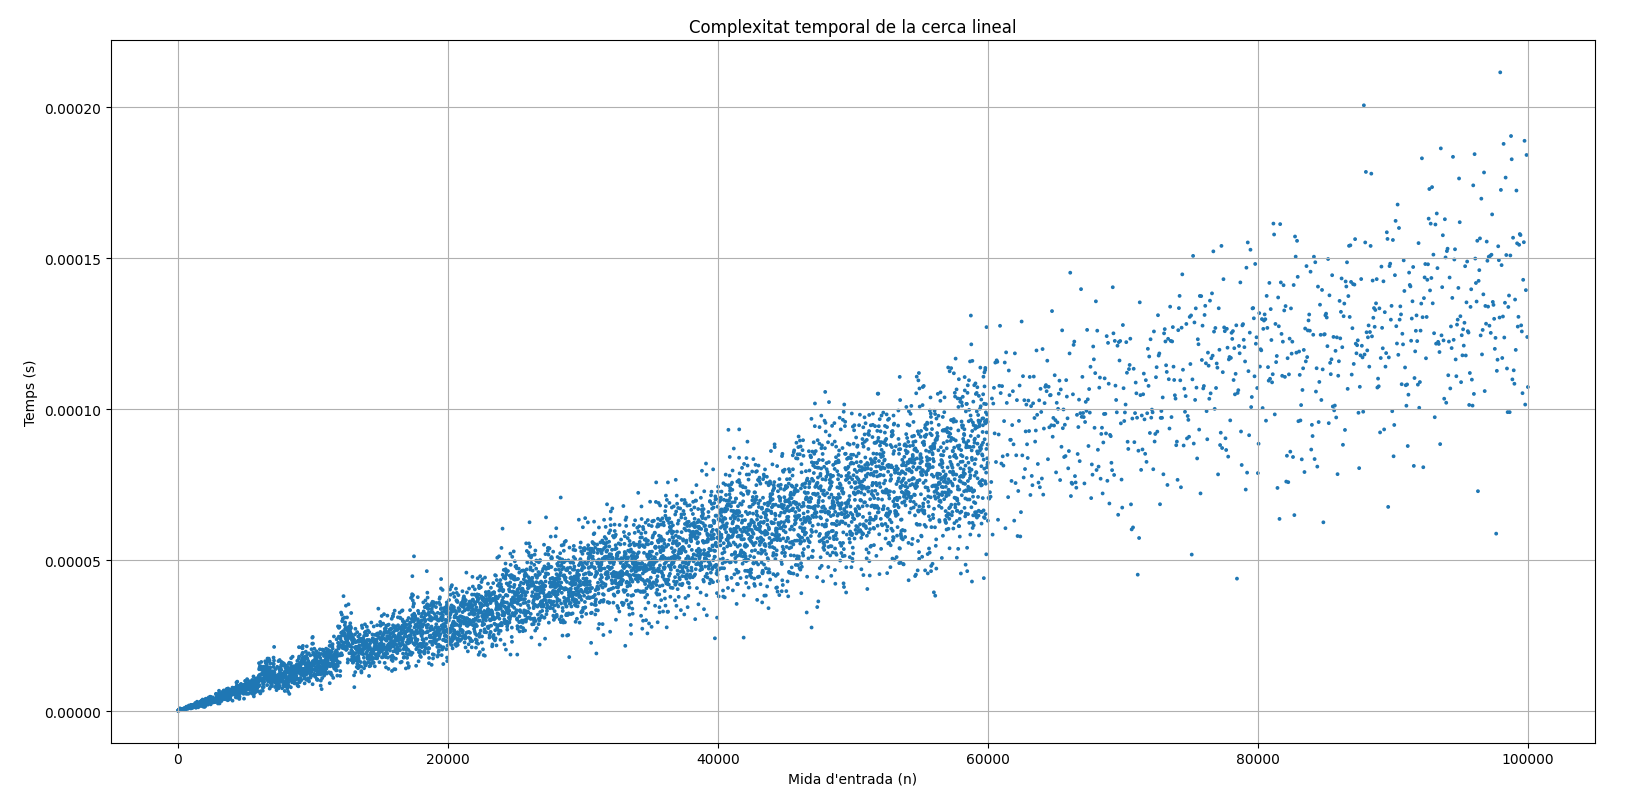
\includegraphics[width=1\textwidth]{capitols/figures/linearplot3.png}
    \caption[Gràfic de dispersió de la cerca lineal.]{Gràfic de dispersió de la cerca lineal. Font: elaboració pròpia.}
    \label{fig:my_label}
\end{figure}

Podem veure en el gràfic de la figura 3.2 una certa relació entre les dues variables. No podem trobar una fórmula que determini el comportament d'aquest programa, ja que hi ha molts factors que afecten els resultats (ordinador, compilador, la dada a cercar...). En canvi, el que podem fer és buscar una correlació entre les dues variables.

En el gràfic 3.2 hi ha una correlació lineal, ja que el gràfic s'aproxima a una recta. Aquesta recta la podem trobar programant amb la llibreria scipy. I obtenim el gràfic 3.3:
\begin{figure}[H]
    \centering
    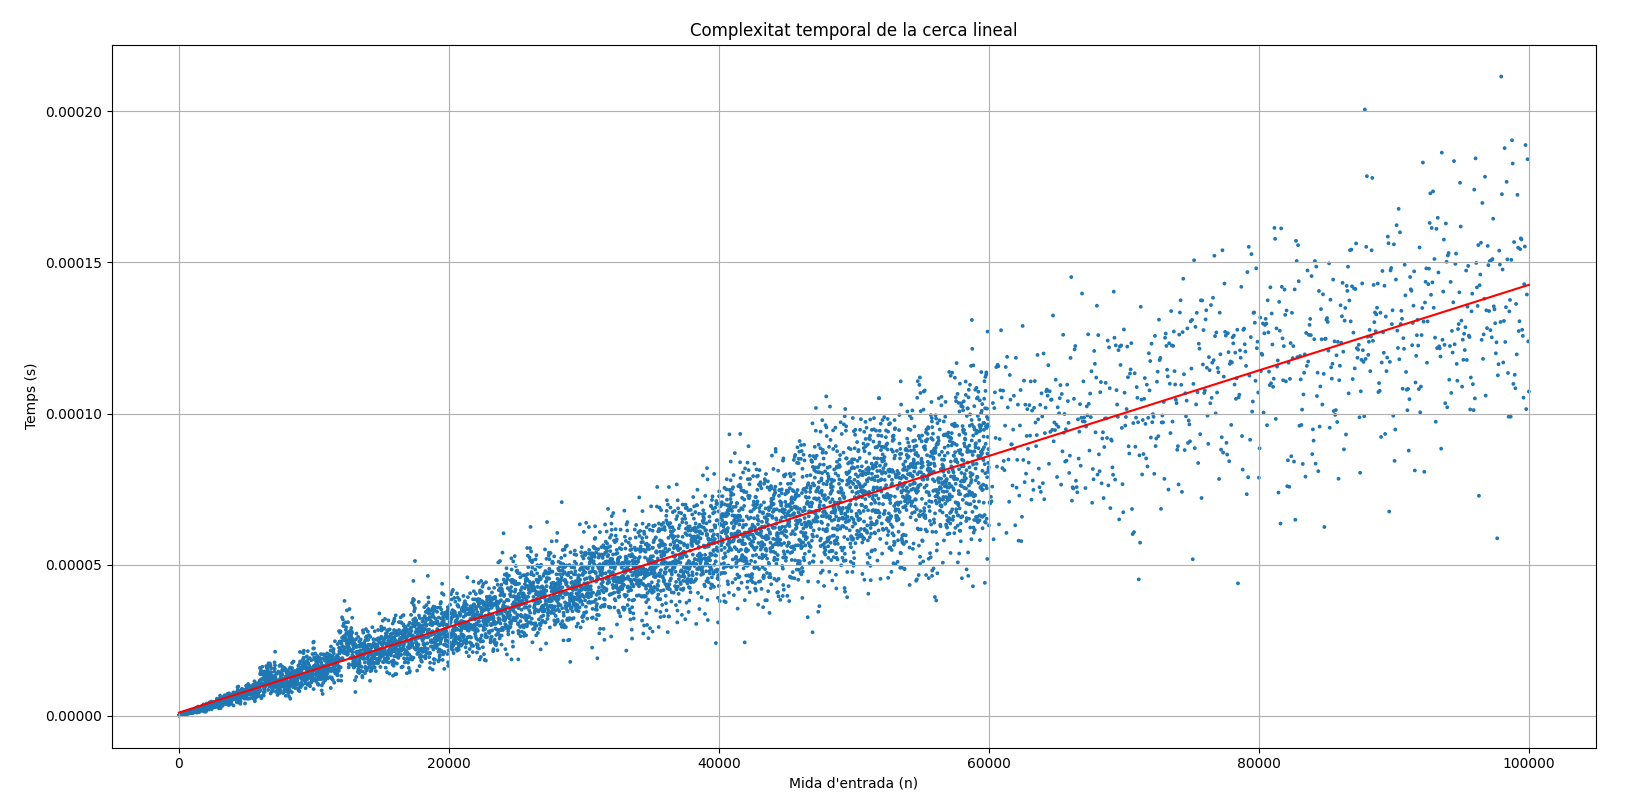
\includegraphics[width=1\textwidth]{capitols/figures/linearplot2.png}
    \caption[Gràfic de dispersió de la cerca lineal amb la recta de correlació lineal.]{Gràfic de dispersió de la cerca lineal amb la recta de correlació lineal. Font: elaboració pròpia.}
    \label{fig:my_label}
\end{figure}

La recta en vermell és la recta que més s'acosta a tots els punts del gràfic.

Si comparem els resultats teòrics que concloïen que la cerca lineal té complexitat $O(n)$ i tornem a fer un gràfic per comparar els resultats.
\begin{figure}[H]
% \vspace{-18pt}
\centering
\begin{tikzpicture}
\centering
\begin{axis}[xmin=0, xmax=200, ymin=0, ymax=400, axis lines = middle, 
x label style={at={(axis description cs:0.5,-0.1)},anchor=north},
y label style={at={(axis description cs:-0.1,.5)},rotate=90,anchor=south},
xlabel={$n$ mida de l'entrada},
ylabel={nombre d'operacions},
style={thick}, 
compat=1.18, width=.4\textwidth, 
% legend style={nodes={scale=0.75, transform shape}}, 
legend pos= south east]
\addplot[color=vermellpral, domain=0:200]{x};
% \addplot[color=verd, domain=0:10]{3*x};
\legend{$O(n)$}
\end{axis}
\end{tikzpicture}
    \caption[Gràfic de complexitat lineal.]{Gràfic de complexitat lineal. Font: elaboració pròpia.}
    \label{fig:my_label}
\end{figure}

Podem veure clarament com els dos gràfics són lineals i, per tant, analitzant la cerca lineal de forma matemàtica i empírica hem arribat al mateix resultat.

En el gràfic 3.4 podem veure que com més creix la mida de l'entrada, les mostres s'allunyen més de la recta. Això és perquè com més gran és la mida de l'entrada, la dada que busquem $k$ pot prendre més valors diferents. És a dir, el programa pot fer entre 1 i $n$ operacions, i com més gran és $n$ més gran és el rang, i per això tenim resultats molt diferents. 

Per comprovar que això és cert, podem executar les mateixes 68.000 mostres per al mateix algoritme, però sent $k$ l'últim element de la llista en tots els casos. D'aquesta manera hem obtingut els següents gràfics:
\begin{figure}[H]
    \centering
    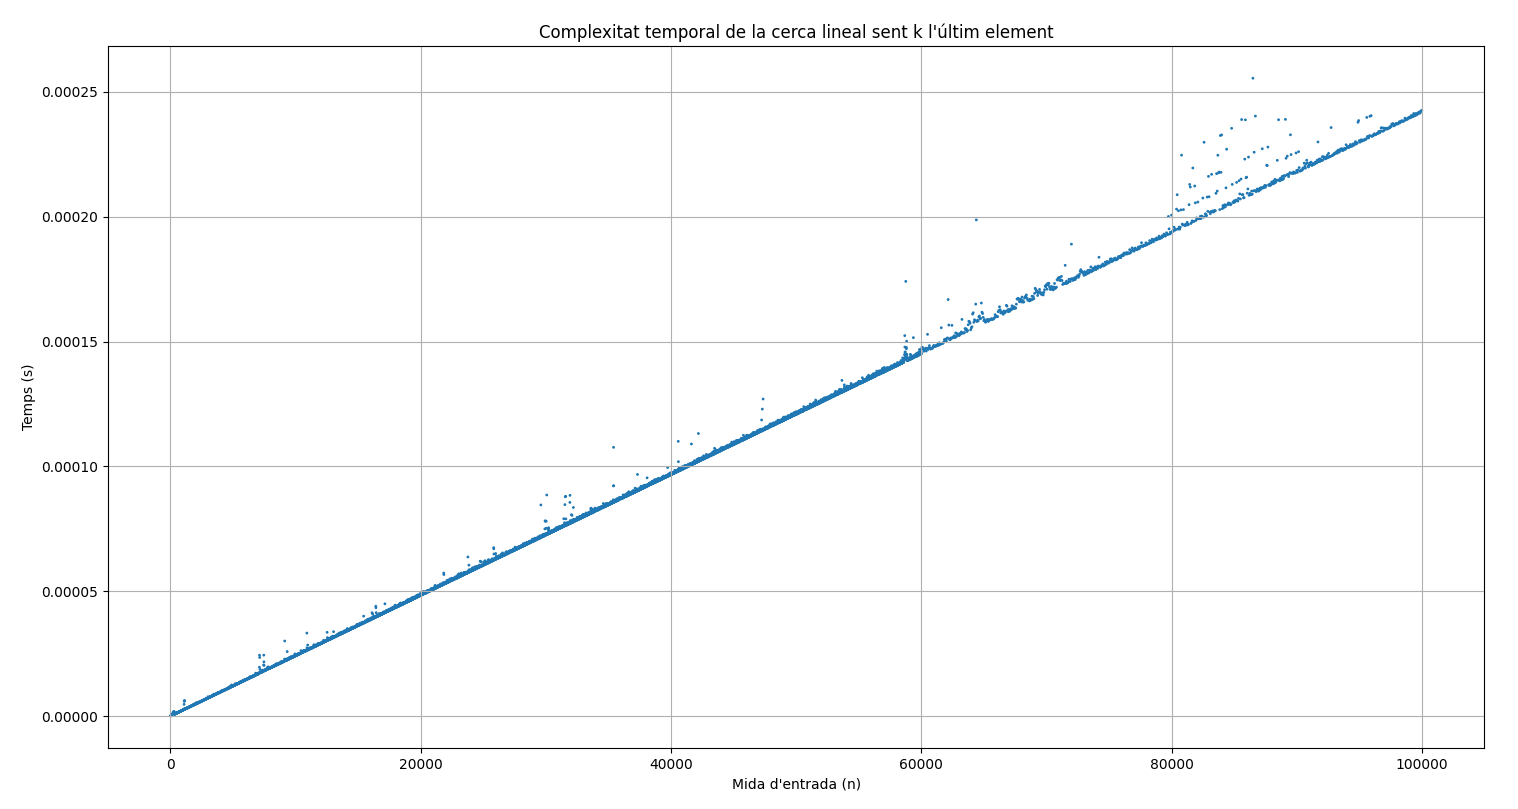
\includegraphics[width=1\textwidth]{capitols/figures/llinerascatter.png}
    \caption[Gràfic de dispersió de la cerca lineal sent $k$ l'últim element.]{Gràfic de dispersió de la cerca lineal sent $k$ l'últim element. Font: elaboració pròpia.}
    \label{fig:my_label}
\end{figure}
\begin{figure}[H]
    \centering
    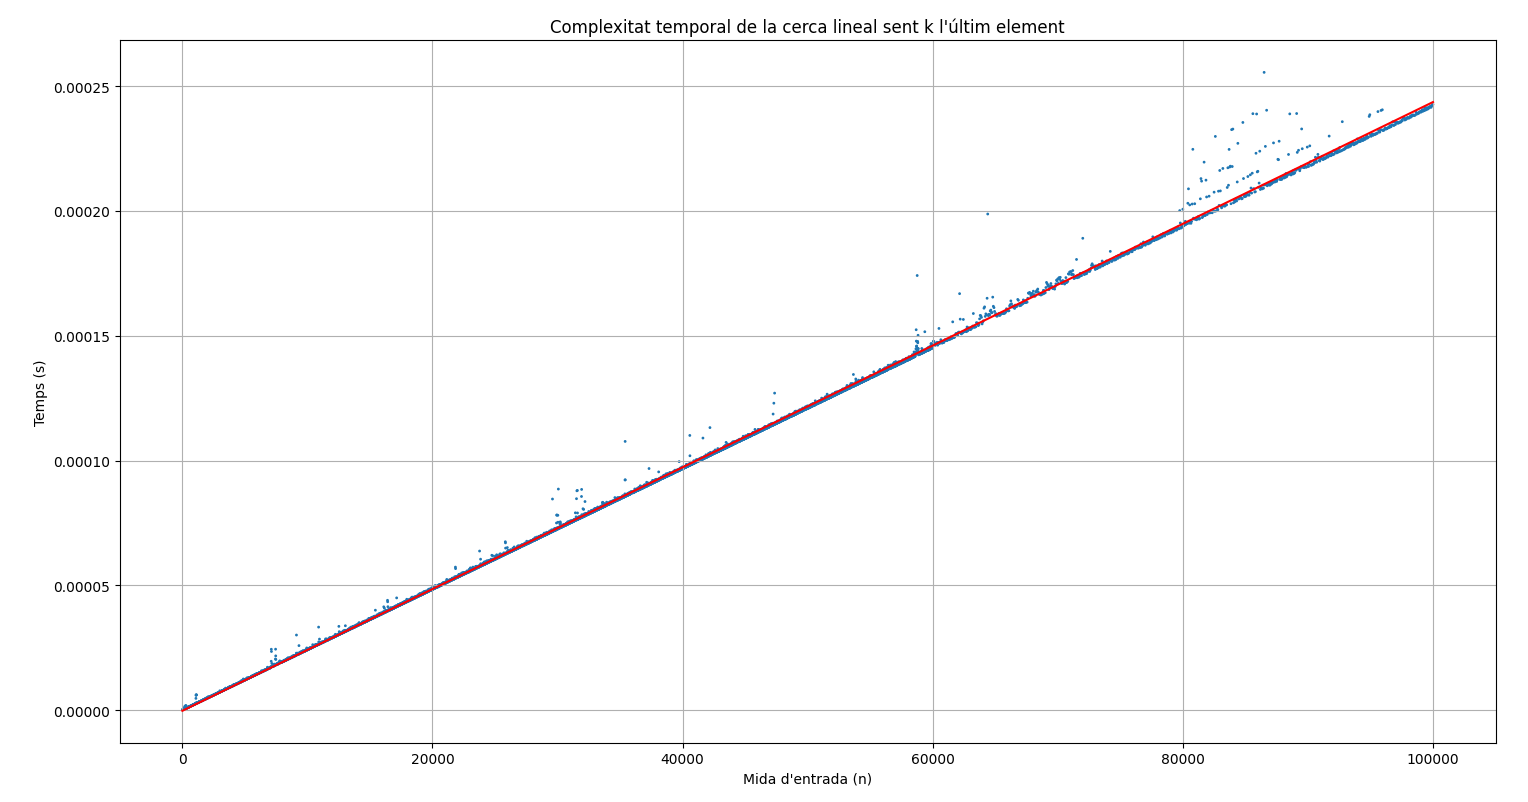
\includegraphics[width=1\textwidth]{capitols/figures/llinearscatterline.png}
    \caption[Gràfic de dispersió de la cerca lineal amb la recta de regressió lineal i sent $k$ l'últim element.]{Gràfic de dispersió de la cerca lineal amb la recta de regressió lineal i sent $k$ l'últim element. Font: elaboració pròpia.}
    \label{fig:my_label}
\end{figure}

En aquests gràfics podem veure de forma més clara que són lineals. A més, la recta de regressió lineal encaixa perfectament amb les mostres que hem obtingut. A més, totes les mostres que s'allunyen de la recta, queden sempre per sobre i mai per sota. Això demostra que quan hi ha hagut algun error, el programa ha tardat més en executar-se i això es pot deure a factors com l'ordinador, sistema operatiu... 

Si comparem els pendents de les rectes, la recta de regressió lineal del gràfic de la figura 3.4 té un pendent de $1.39748 \cdot 10^9$ i la recta del gràfic de la figura 3.7 té un pendent de $2.43812 \cdot 10^9$. És correcte que el pendent de la recta que hem obtingut en l'algoritme en què hem executat el pitjor cas possible sigui superior que en el cas en què $k$ era aleatori. 

Així que podríem tornar a executar l'algoritme en un tercer cas en què $k$ es trobi sempre al centre. D'aquesta manera hauríem d'obtenir una recta més semblant a la de la figura 3.4, però amb els resultats molt més propers a la recta, com en la figura 3.7.

Hem obtingut els següents gràfics:
\begin{figure}[H]
    \centering
    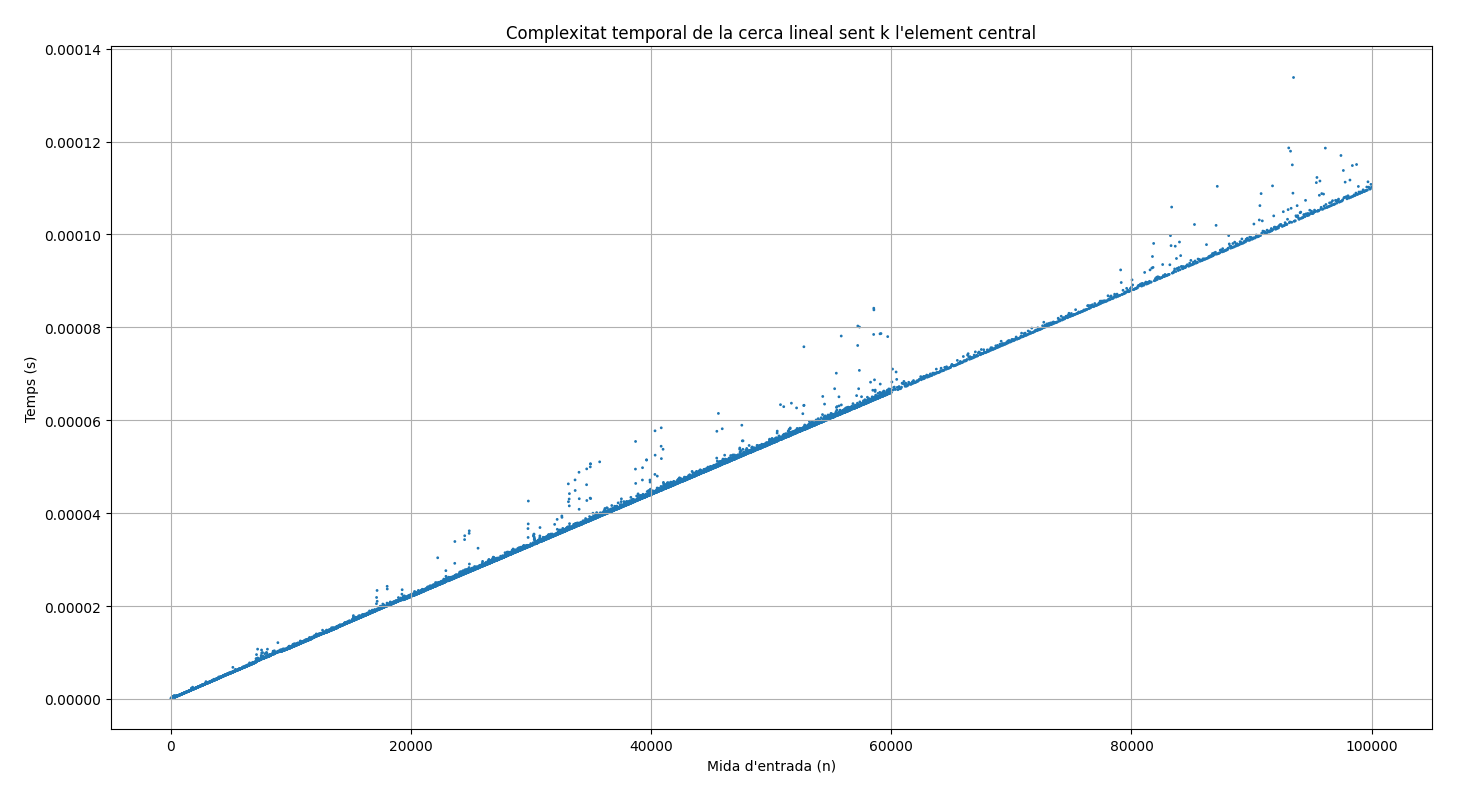
\includegraphics[width=1\textwidth]{capitols/figures/linearmidscatter.png}
    \caption[Gràfic de dispersió de la cerca lineal sent $k$ l'element central.]{Gràfic de dispersió de la cerca lineal sent $k$ l'element central. Font: elaboració pròpia.}
    \label{fig:my_label}
\end{figure}
\begin{figure}[H]
    \centering
    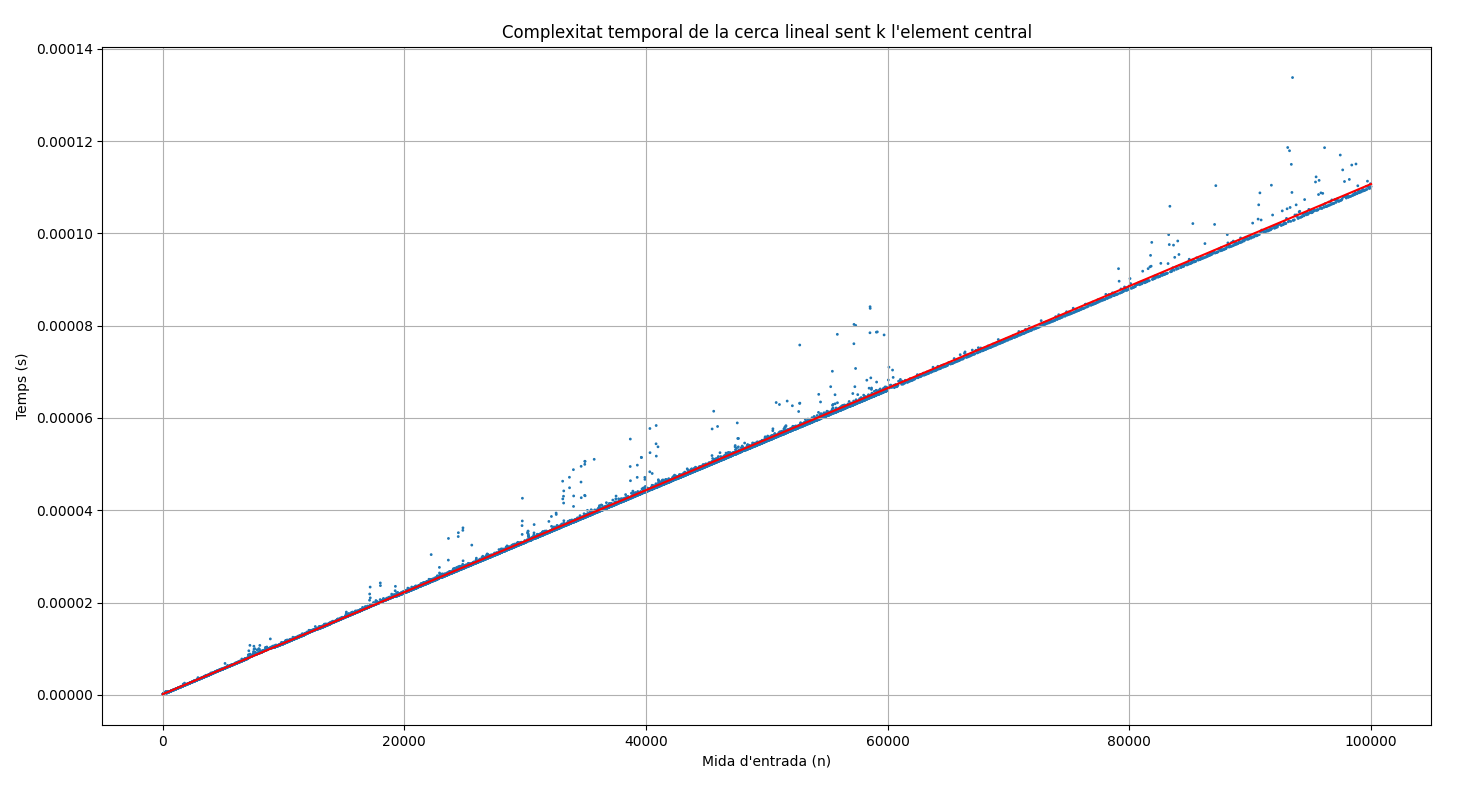
\includegraphics[width=1\textwidth]{capitols/figures/linearmidscatterline.png}
    \caption[Gràfic de dispersió de la cerca lineal amb la recta de regressió lineal i sent $k$ l'element central.]{Gràfic de dispersió de la cerca lineal amb la recta de regressió lineal i sent $k$ l'element central. Font: elaboració pròpia.}
    \label{fig:my_label}
\end{figure}

El pendent de la recta del gràfic de la figura 3.9 és d'$1.10601 \cdot 10^9$ el qual s'aproxima al de la recta del gràfic 3.4 i les mostres són molt més properes a la recta, com havíem predit.

\subsubsection{Anàlisi empíric de la cerca dicotòmica}
Ja que aquest algoritme és més eficient que el de la cerca lineal, he pogut recopilar més mostres. He executat l'algoritme 401.610 vegades. L'he executat 10 vegades per cada mida d'entrada entre 10 i 200.000 en intervals de 10 unitats. Com que entre l'interval d'entre 1 i 10.000 hi havia molt d'error, he recopilat més mostres.

Finalment he obtingut els següents gràfics:
\begin{figure}[H]
    \centering
    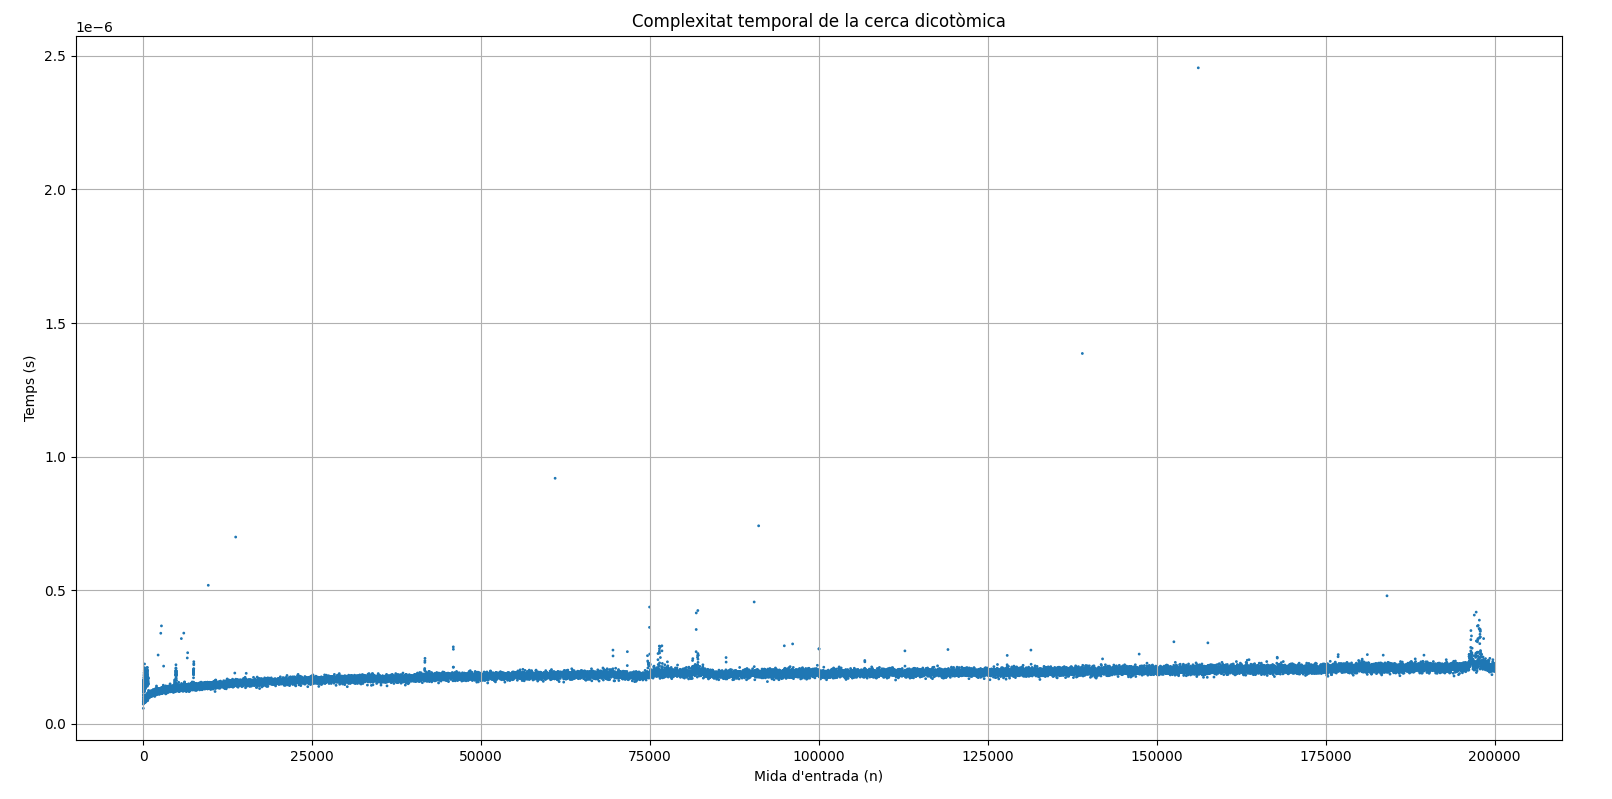
\includegraphics[width=1\textwidth]{capitols/figures/dicotomicagrafic.png}
    \caption[Gràfic de dispersió de la cerca dicotòmica.]{Gràfic de dispersió de la cerca dicotòmica. Font: elaboració pròpia.}
    \label{fig:my_label}
\end{figure}
\begin{figure}[H]
    \centering
    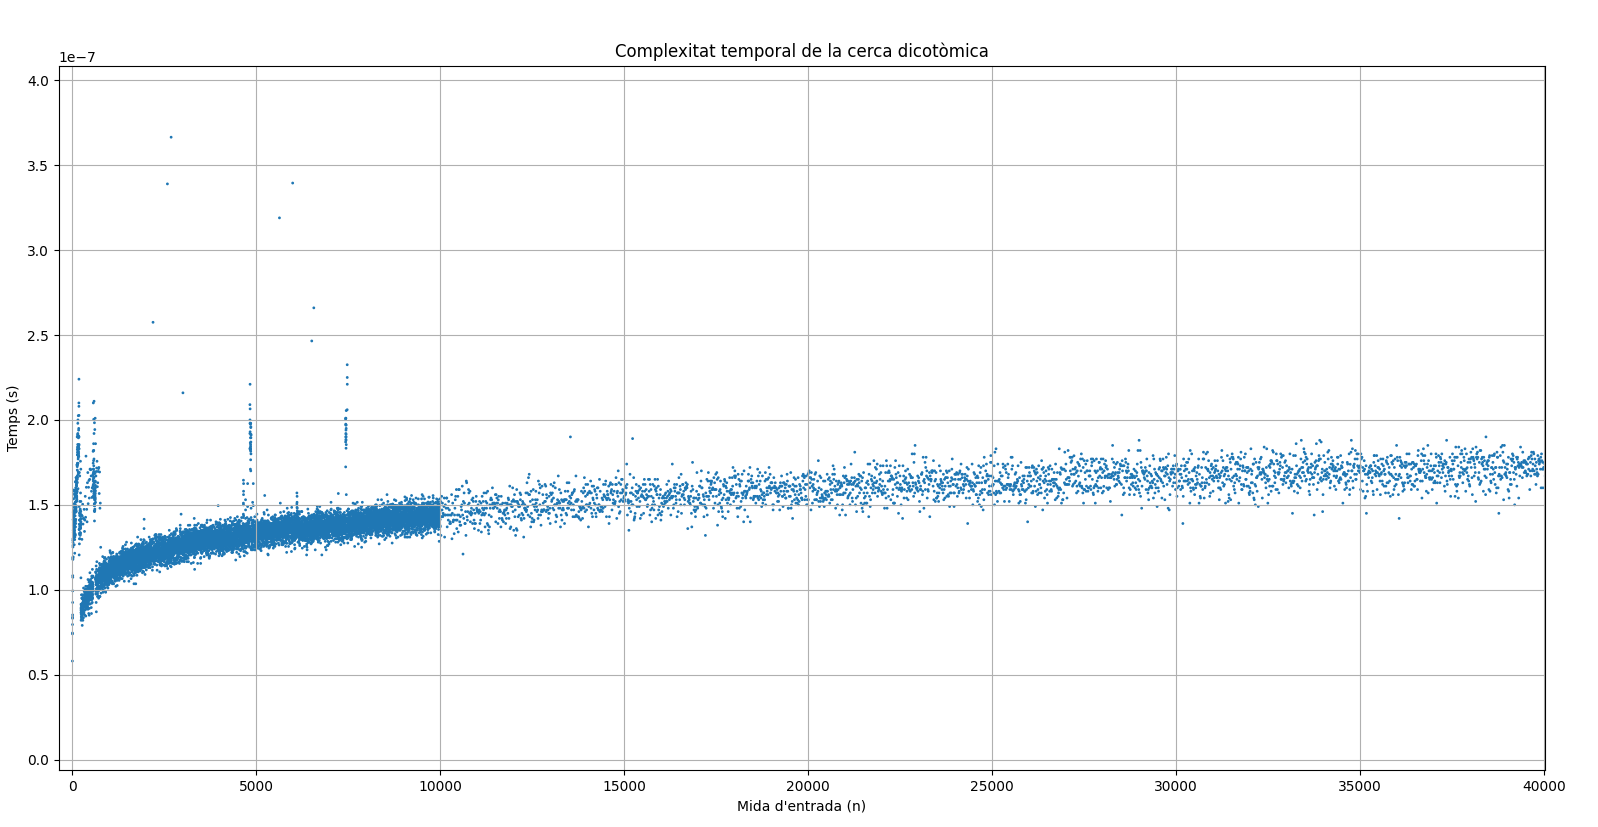
\includegraphics[width=1\textwidth]{capitols/figures/dicotomicaampliat.png}
    \caption[Gràfic de dispersió de la cerca dicotòmica entre l'interval 1 - 40.000.]{Gràfic de dispersió de la cerca dicotòmica entre l'interval 1 - 40.000. Font: elaboració pròpia.}
    \label{fig:my_label}
\end{figure}
\begin{figure}[H]
    \centering
    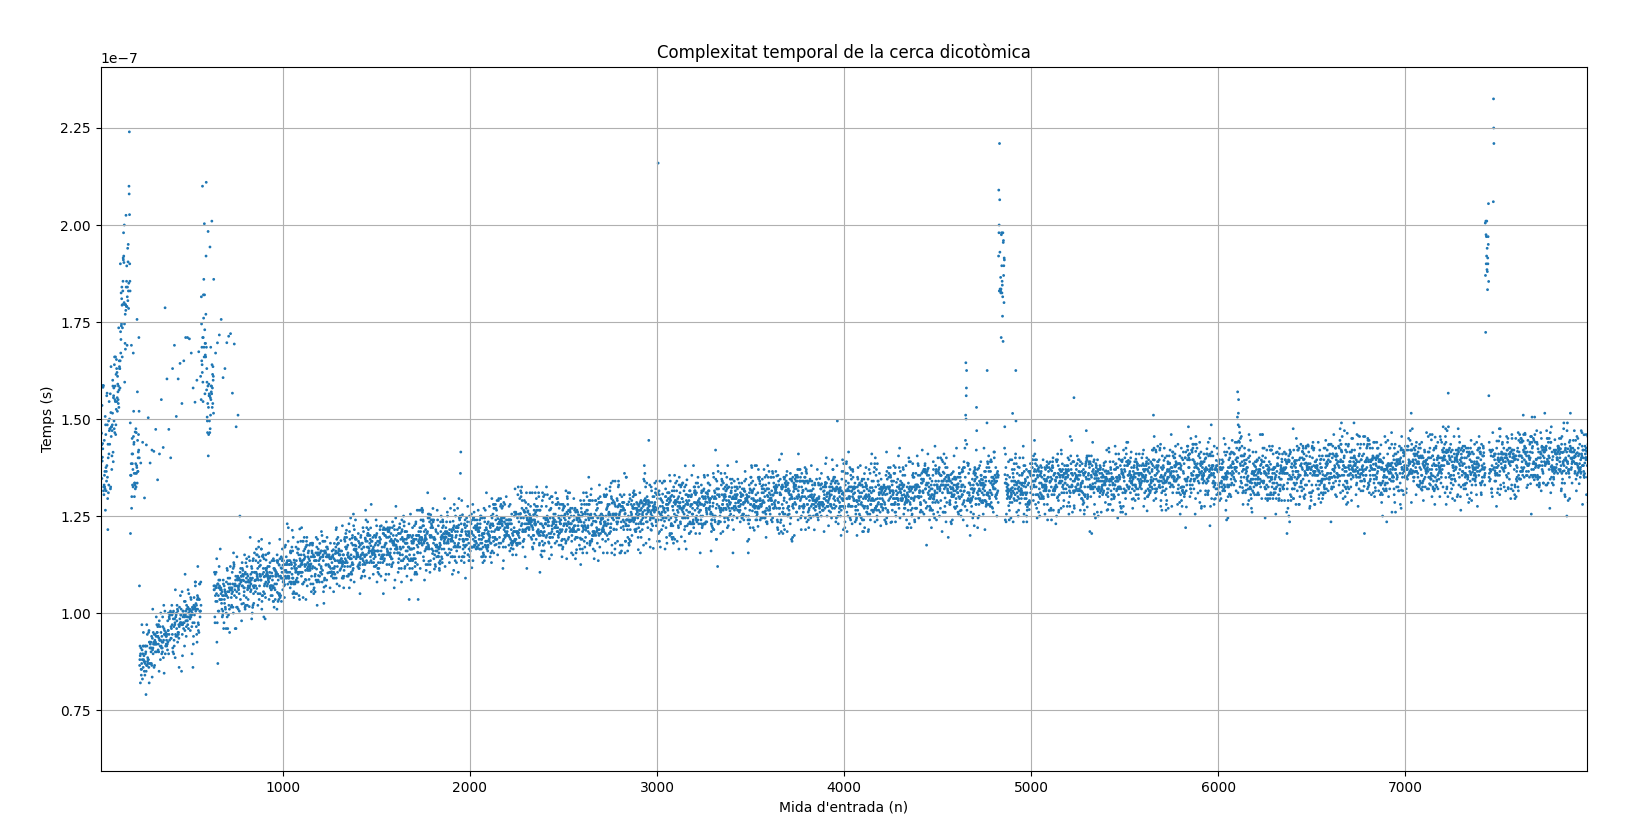
\includegraphics[width=1\textwidth]{capitols/figures/zoomin.png}
    \caption[Gràfic de dispersió de la cerca dicotòmica entre l'interval 1 - 8.000.]{Gràfic de dispersió de la cerca dicotòmica entre l'interval 1 - 8.000. Font: elaboració pròpia.}
    \label{fig:my_label}
\end{figure}

Podem veure que aquests gràfics tenen la mateixa forma que la funció logarítmica.

\begin{figure}[H]
    \centering
    % \vspace{-18pt}
\begin{tikzpicture}
\centering
\begin{axis}[xmin=0, xmax=300, ymin=0, ymax=40, axis lines = middle, 
x label style={at={(axis description cs:0.5,-0.1)},anchor=north},
y label style={at={(axis description cs:-0.1,.5)},rotate=90,anchor=south},
xlabel={$n$ mida de l'entrada},
ylabel={nombre d'operacions},
style={thick}, 
compat=1.18, width=.4\textwidth]
\addplot[color=vermellpral, domain=-2:300, samples=150]{log2(x)};
\legend{$O(\log_2{n})$}
\end{axis}
\end{tikzpicture}
    \caption[Complexitat logarítmica.]{Complexitat logarítmica. Font: elaboració pròpia.}
    \label{fig:my_label}
\end{figure}

Si comparem els gràfics de les figures 3.8 i 3.9 podem veure que els dos tenen la mateixa forma. Per tant, hem demostrat de forma pràctica i teòrica que la cerca dicotòmica té complexitat logarítmica.

També podem veure que en aquests gràfics les mostres no s'allunyen tant com en la cerca lineal, així que podem arribar a la conclusió que la posició de $k$ no afecta gaire els resultats, tampoc quan la mida de l'entrada és molt gran.

\subsubsection{Anàlisi empíric de l'ordenació de bombolla}
Aquest algoritme l'he executat 15.837 vegades. L'he executat 10 vegades per cada mida d'entrada entre 1 i 8.000 en intervals de deu unitats, i 10 vegades entre 8.000 i 10.000 en intervals de 50 unitats.

He obtingut els següents gràfics:
\begin{figure}[H]
    \centering
    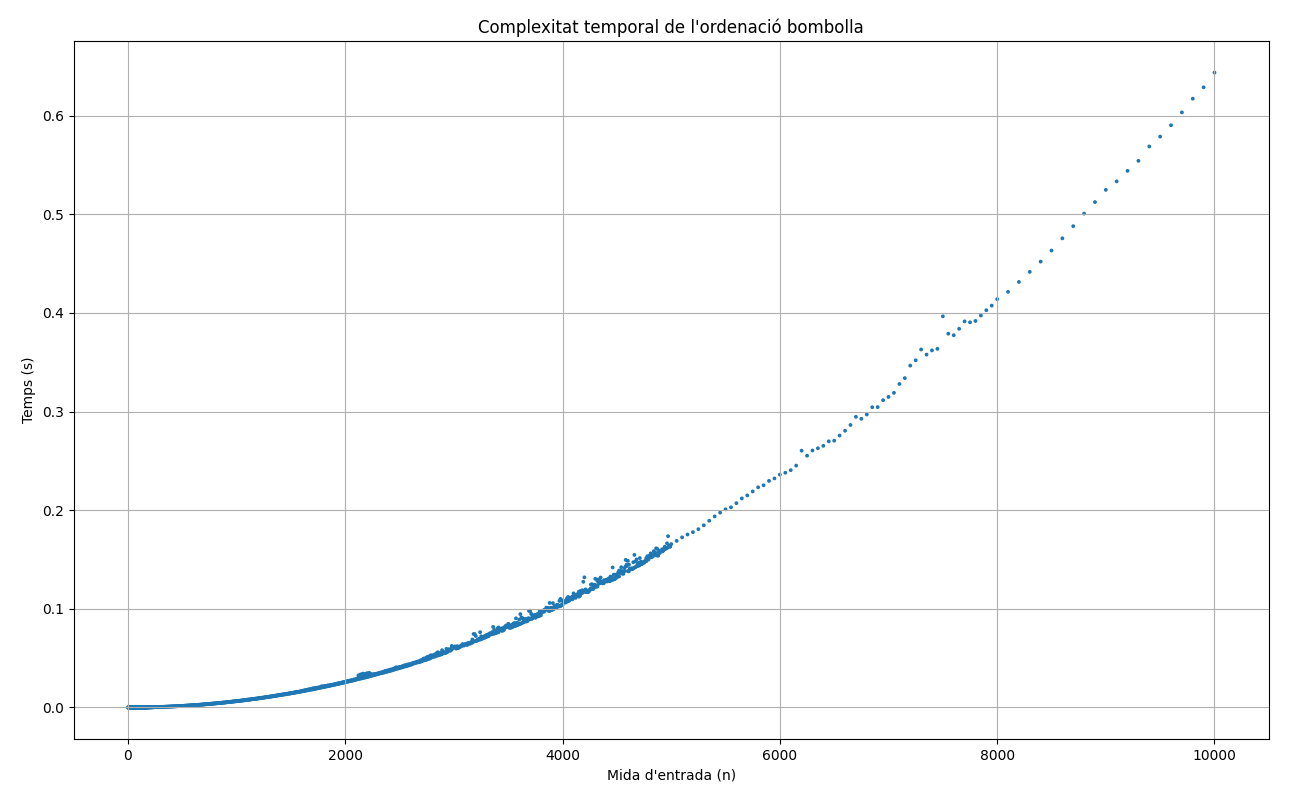
\includegraphics[width=1\textwidth]{capitols/figures/bombollascater2.png}
    \caption[Gràfic de dispersió de l'ordenació bombolla.]{Gràfic de dispersió de l'ordenació bombolla. Font: elaboració pròpia.}
    \label{fig:my_label}
\end{figure}
\begin{figure}[H]
    \centering
    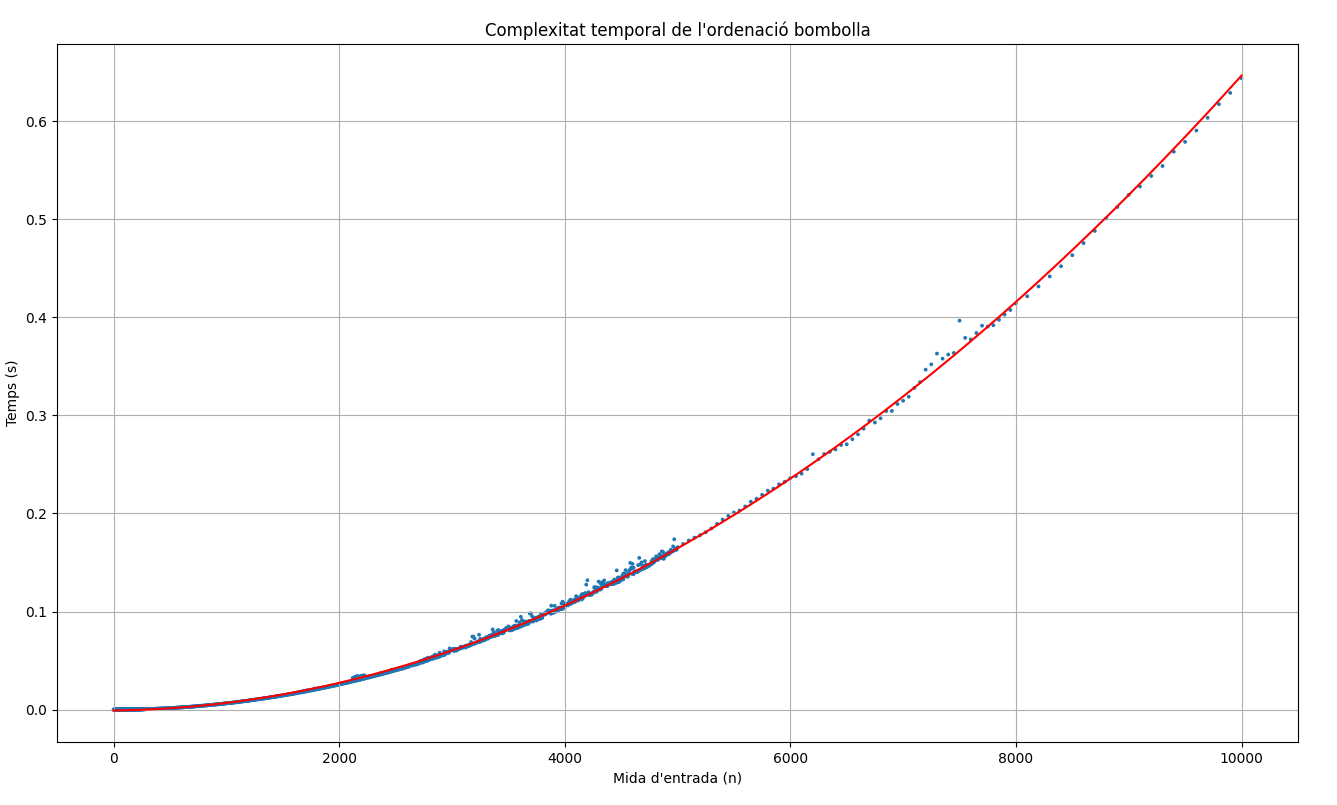
\includegraphics[width=1\textwidth]{capitols/figures/bombollascaterline.png}
    \caption[Gràfic de dispersió de l'ordenació bombolla amb la corba de regressió $f(x) = 6.33 \cdot 10^{-9} x^2 + 1.4 \cdot 10^{-6} x - 0.0008552$.]{Gràfic de dispersió de l'ordenació bombolla amb la corba de regressió $f(x) = 6.33 \cdot 10^{-9} x^2 + 1.4 \cdot 10^{-6} x - 0.0008552$. Font: elaboració pròpia.}
    \label{fig:my_label}
\end{figure}

% \vspace{-18pt}

Podem veure clarament que la forma que té el gràfic de la figura 3.10 s'assembla molt a la funció quadràtica. A més, encaixa perfectament amb la corba de regressió polinòmica.

\begin{figure}[H]
    \centering
    % \vspace{-18pt}
\begin{tikzpicture}
\centering
\begin{axis}[xmin=0, xmax=25, ymin=0, ymax=700, axis lines = middle, 
x label style={at={(axis description cs:0.5,-0.1)},anchor=north},
y label style={at={(axis description cs:-0.1,.5)},rotate=90,anchor=south},
xlabel={$n$ mida de l'entrada},
ylabel={nombre d'operacions},
style={thick}, 
compat=1.18, width=.4\textwidth, 
% legend style={nodes={scale=0.75, transform shape}}, 
legend pos=south east]
\addplot[color=vermellpral, domain=0:25, samples=150]{x^2};
% \addplot[color=verd, domain=0:10]{2*(x^2)};
\legend{$O(n^2)$, $O(2 \cdot n^2)$}
\end{axis}
\end{tikzpicture}
    \caption[Gràfic de complexitat quadràtica.]{Gràfic de complexitat quadràtica. Font: elaboració pròpia.}
    \label{fig:my_label}
\end{figure}

Per tant, amb l'estudi matemàtic i empíric hem arribat a la mateixa conclusió: l'ordenació bombolla té complexitat quadràtica.

\subsubsection{Anàlisi empíric de l'ordenació per barreja}
Aquest algoritme l'he executat 54.260 vegades. Ho he fet 10 vegades per cada mida d'entrada d'entre 10 i 30.000 en intervals de 10 unitats, de 30.050 a 100.000 en intervals de 50 unitats i de 100.100 a 200.000 en intervals de 100 unitats. També he reforçat amb més mostres les parts del gràfic que s'allunyaven més de la resta de mostres.

Finalment he obtingut el següent gràfic:
\begin{figure}[H]
    \centering
    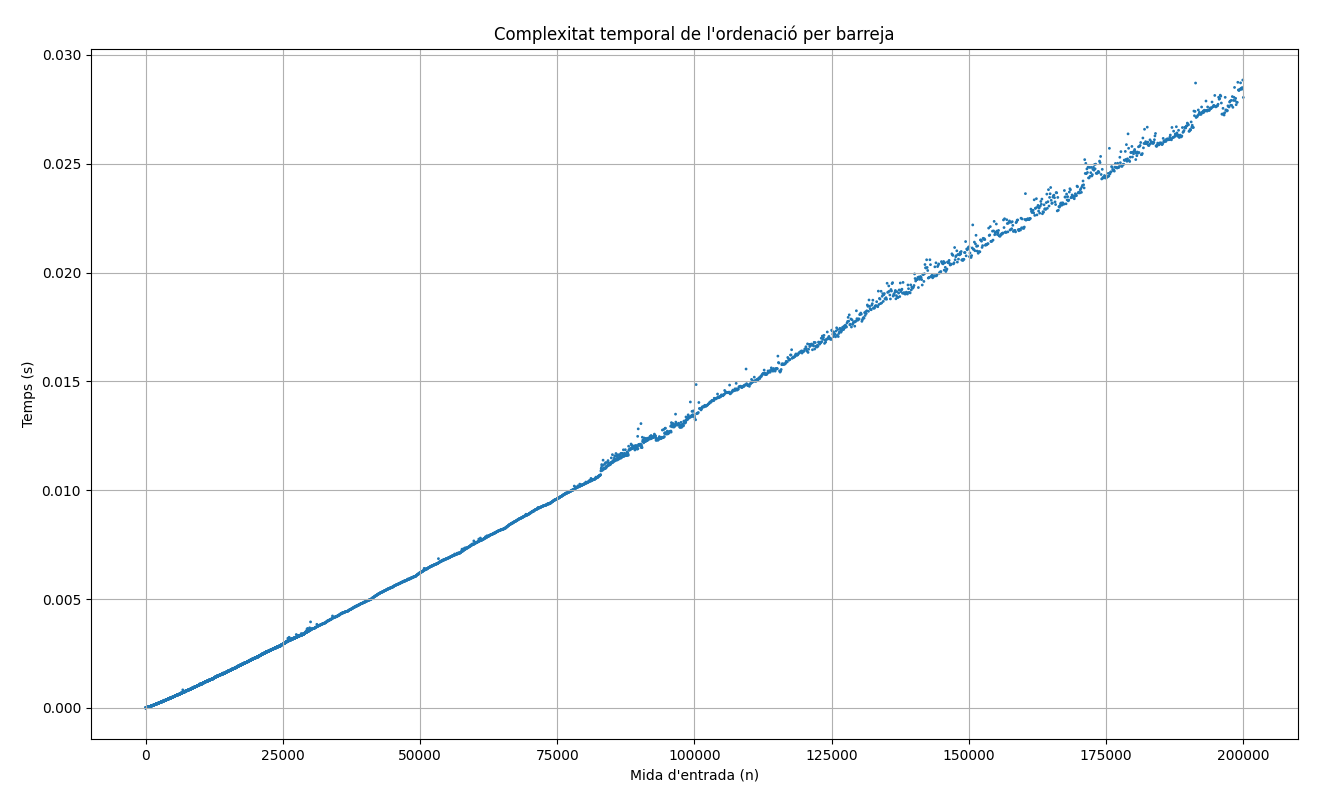
\includegraphics[width=1\textwidth]{capitols/figures/mergescatter.png}
    \caption[Gràfic de dispersió de l'ordenació per barreja.]{Gràfic de dispersió de l'ordenació per barreja. Font: elaboració pròpia.}
    \label{fig:my_label}
\end{figure}
\vspace{-18pt}
Sembla una recta així que podríem dibuixar al gràfic una recta de regressió lineal:
\begin{figure}[H]
    \centering
    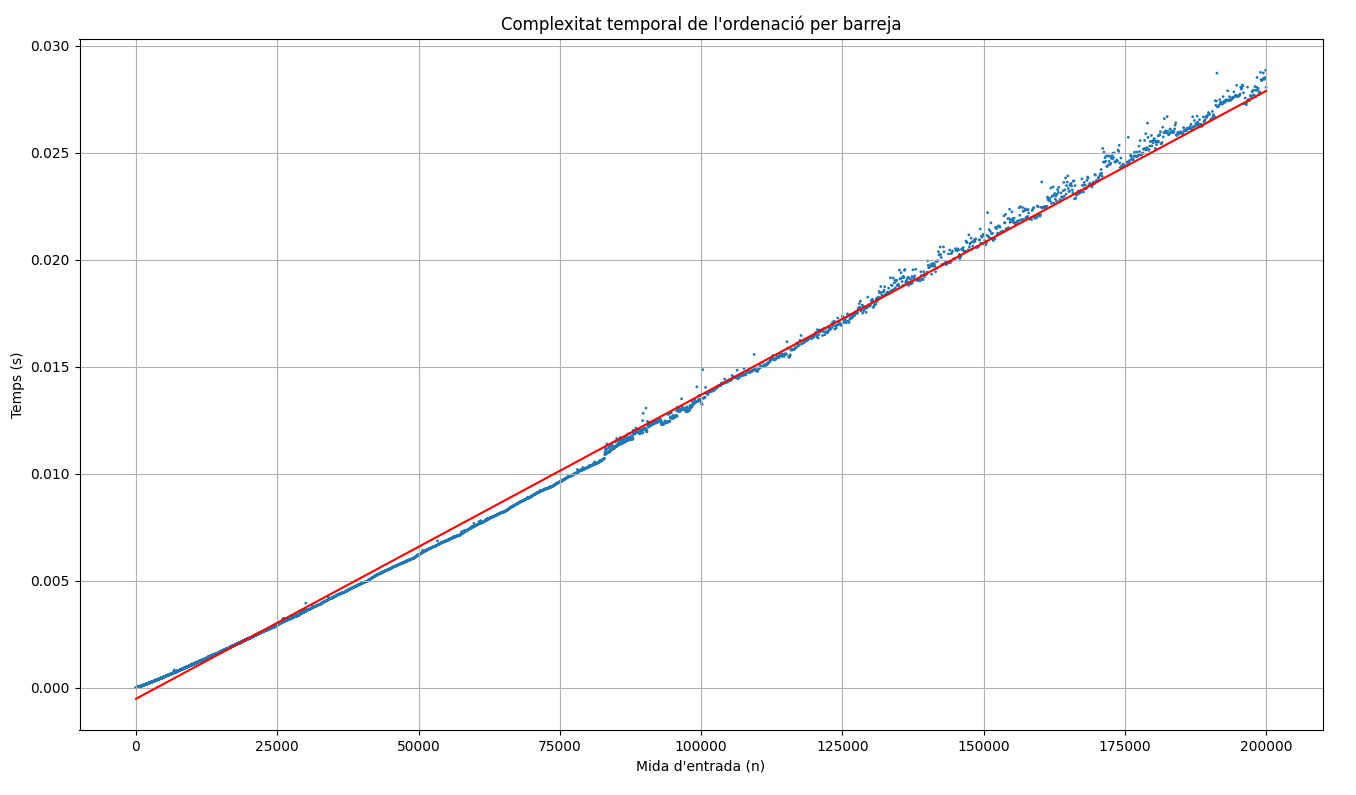
\includegraphics[width=1\textwidth]{capitols/figures/mergescaterline.png}
    \caption[Gràfic de dispersió de l'ordenació per barreja amb la recta de regressió lineal.]{Gràfic de dispersió de l'ordenació per barreja amb la recta de regressió lineal. Font: elaboració pròpia.}
    \label{fig:my_label}
\end{figure}

Si comparem la recta vermella amb les dades que hem obtingut, podem veure que no acaba d'encaixar.

En l'anàlisi matemàtic hem arribat a la conclusió que aquest algoritme té complexitat $O(n \cdot \log_2{n})$. Així que podem comparar les figures 3.12 i 3.14.
\begin{figure}[H]
    \centering
    % \vspace{-18pt}
\begin{tikzpicture}
\centering
\begin{axis}[xmin=0, xmax=25, ymin=0, ymax=150, axis lines = middle, 
x label style={at={(axis description cs:0.5,-0.1)},anchor=north},
y label style={at={(axis description cs:-0.1,.5)},rotate=90,anchor=south},
xlabel={$n$ mida de l'entrada},
ylabel={nombre d'operacions},
style={thick}, 
compat=1.18, width=.4\textwidth, 
legend style={nodes={scale=0.8, transform shape}}, 
legend pos=south east]
\addplot[color=vermellpral, domain=0:25, samples=150]{x*log2(x)};
% \addplot[color=verd, domain=0:10]{2*(x^2)};
\legend{$O(n \cdot \log_2{n})$}
\end{axis}
\end{tikzpicture}
    \caption[Gràfic de complexitat $O(n \cdot \log_2{n})$.]{Gràfic de complexitat $O(n \cdot \log_2{n})$. Font: elaboració pròpia.}
    \label{fig:my_label}
\end{figure}

Podem veure com els gràfics s'assemblen, encara que no tant com en els altres tres algoritmes. 


En aquest gràfic i el de la cerca dicotòmica no he trobat la recta de regressió, ja que és més complicat quan les funcions són logarítmiques.